\documentclass[twocolumn]{article}
\usepackage{lipsum}  % This package generates filler text.
\usepackage{amsmath} % For mathematical formulas.
\usepackage{graphicx} % For including figures.
\usepackage{authblk} % For author and affiliation blocks.
\usepackage[english]{babel}
\usepackage{graphicx} % Required for inserting images
\usepackage{subcaption}
\usepackage{algorithm}
\usepackage{algpseudocode}
\usepackage[T1]{fontenc}
\usepackage[utf8]{inputenc}
\usepackage{url}
\usepackage{hyperref}
\usepackage{parskip}
\usepackage{xcolor}
\usepackage[margin=1in]{geometry}
\usepackage{amssymb}
\usepackage{comment}
\usepackage{multicol}
\usepackage{svg}

\hypersetup{
    colorlinks=true,
    urlcolor=blue
}

\newcommand{\C}{\mathbb{C}}
\newcommand{\R}{\mathbb{R}}
\newcommand{\Q}{\mathbb{Q}}
\newcommand{\Z}{\mathbb{Z}}
\newcommand{\N}{\mathbb{N}}
\newcommand{\proofend}{\hfill $\square$}
\newcommand{\deltach}{\hat{\delta}}

\title{STT 3795: Report}
\author{Bio Samir Gbian: 20250793}
\author{Kamen Damov: 20102811}
\author{Simon Langlois: 20247696}
\affil{Department of Mathematics and Statistics}
\affil{University of Montreal}

\begin{document}
\maketitle

\section{Introduction}
Language classification is a crucial task in many fields, from natural language technology to speech recognition and machine translation. The rise of big data and the diversity of languages spoken around the world have amplified the importance of having effective classification methods to process and analyze these data meaningfully.

In this context, evaluating and comparing the performance of classification algorithms is essential to identify the most suitable approaches for this complex task. This project aims to examine and compare the quality of some of the most commonly used classification algorithms in language classification. In particular, we focus on evaluating the performance of Support Vector Machines (SVM) and Random Forests.

\section{Objectives}
The main objective of this project is to identify the strengths and weaknesses of each classification algorithm in the specific context of language classification. To achieve this, we will use representative datasets containing voice samples from different people, covering a variety of linguistic structures and features. We will assess the performance of each algorithm in terms of accuracy, recall, F-measure, \textbf{and other quality metrics of classification}.

\section{Description of Analyzed Data}
\subsection{Source}
The data used in the project comes from the \textit{Hugging Face} website. It is a reliable internet site for hosting datasets as well as sharing pre-trained AI models. This allows us to have a reference to compare our model to, which is one of the main reasons why this dataset was chosen.
The dataset, named \textit{Common Language}, contains several audio files in WAV format (specifically 34045 files). These files are separated into three types: training, testing, and validation. Each audio represents a person of a certain gender (Male/Female) quoting a phrase or repeating words in a language. Forty-five different languages are spoken in these audios (See source in reference for more details on all the languages spoken).

\subsection{Data Cleaning}
The initial raw data attributes are: Client id, Path (Link to the audio file), Age (Speaker's age), Gender(Speaker's gender) and the language spoken in the audio.\\

Given that our project was solely focused on the classification of the spoken languages, We removed all the columns except the paths to the \text{Language} (our target label), and \text{Path} (the paths to the raw wav files containing the spoken languages). After listening to some audio files and plotting the spectral representation of the audio, we realized that most wav files had a few seconds of silence or some background sounds that weren't spoken language. In order to have data that is exclusively spoken language sound waves on which our classification models would be trained on, we have to remove the non-spoken language sounds (see Algorithm 1).  
\begin{algorithm}
\caption{Audio Cleaning Process}
\begin{algorithmic}[1]
\State Initialize paths for raw and cleaned audio files
\State Prepare empty list for errors
\Function{clean\_sound}{audio}
    \State Define threshold to identify significant audio (e.g., 1\%)
    \State Find the start and end of significant audio using the threshold
    \State Trim the audio outside the significant range
    \State \Return the trimmed audio
\EndFunction
\For{each audio file in the dataset}
        \State Read the audio file to obtain waveform data
        \State Apply noise reduction to the waveform
        \Try
            \State Clean the audio using the clean\_sound function
            \State Save the cleaned audio to the designated output path
        \Except
            \State Log error with file details
        \EndTry
\end{algorithmic}
\end{algorithm}

As we can see in Figure 1 and Figure 2, only relevant data has been kept, as the white noise has been removed. The new shape obtained contains less noise than the first shape. This allows for more reliable data. However, there are some data in which the extremities are significant but will still be removed. Therefore, globally, the data are more reliable but we lose information.\\
\begin{figure}[!tbp]
  \centering
  \begin{minipage}[b]{0.4\textwidth}
    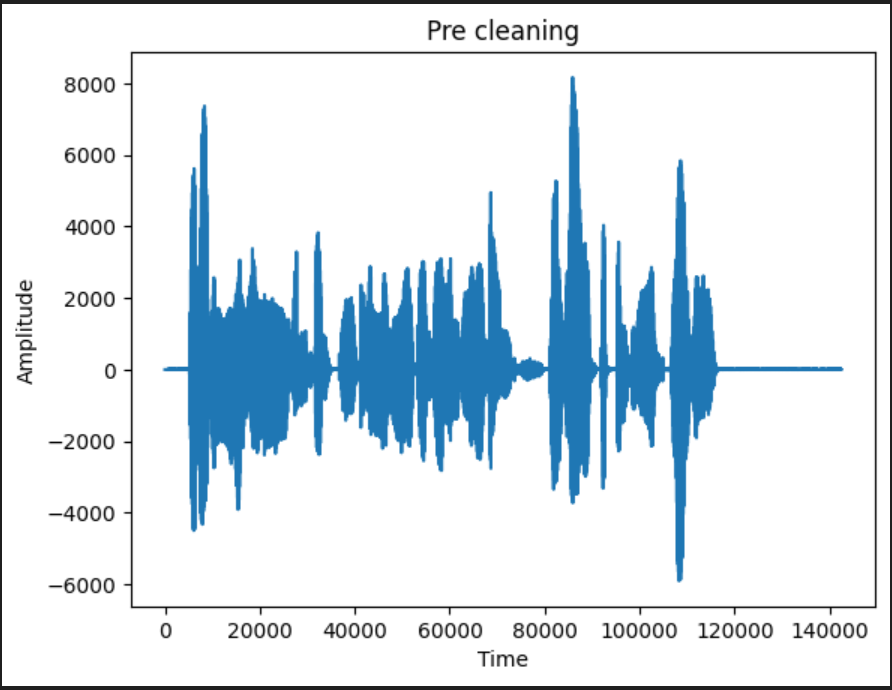
\includegraphics[width=\textwidth]{images/pre_cleaning.png}
    \caption{Pre cleaning shape}
  \end{minipage}
  \hfill
  \begin{minipage}[b]{0.4\textwidth}
    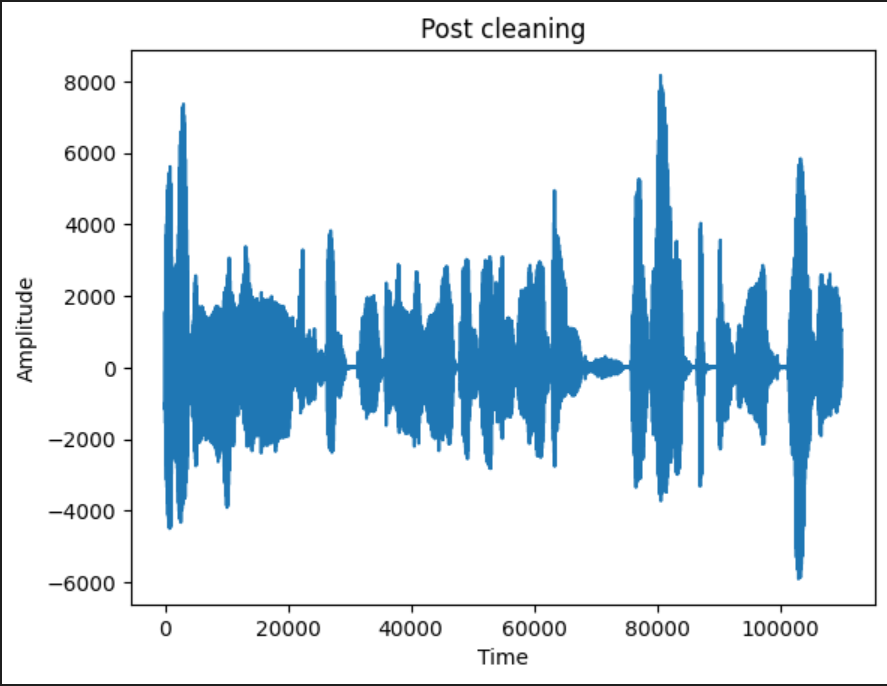
\includegraphics[width=\textwidth]{images/post_cleaning.png}
    \caption{Post cleaning shape}
  \end{minipage}
\end{figure}

\subsection{Statistics}
Before preprocessing our audio data into features for model training, we need to verify that the data is well-balanced across various attributes, such as label distribution, category balance, and uniformity in audio lengths. We looked at three statistics on the data: the number of audio files by language (Figure 3 (a)), the average length of audios by language (Figure 3 (b)), and the total length of audios by language (Figure 3 (c)). 
\begin{figure}[h]
    \centering
    \begin{subfigure}[b]{0.3\textwidth}
        \centering
        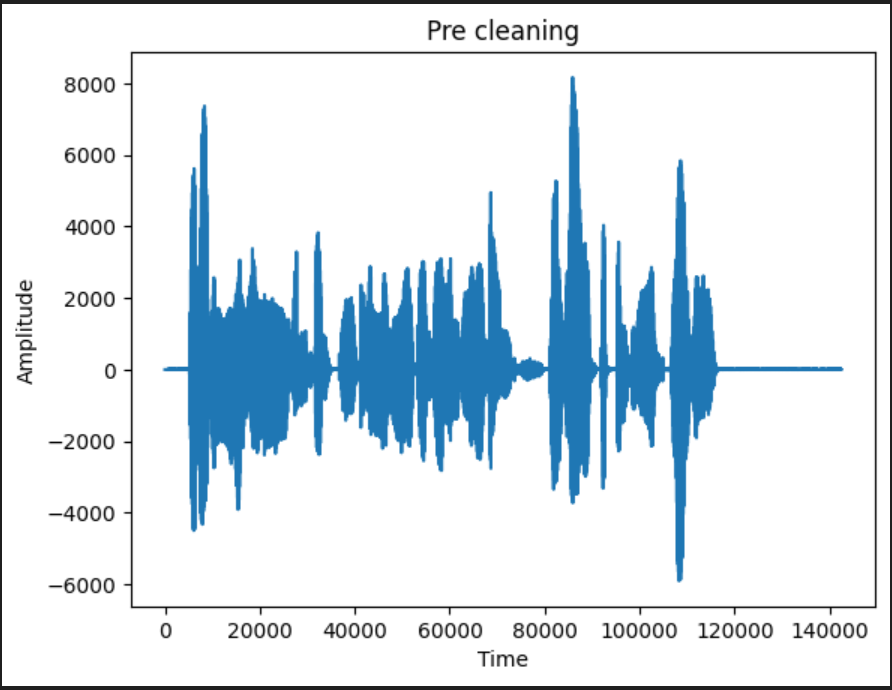
\includegraphics[width=\linewidth]{images/pre_cleaning.png}
        \caption{Figure 1}
        \label{fig:image1}
    \end{subfigure}
    \hfill
    \begin{subfigure}[b]{0.3\textwidth}
        \centering
        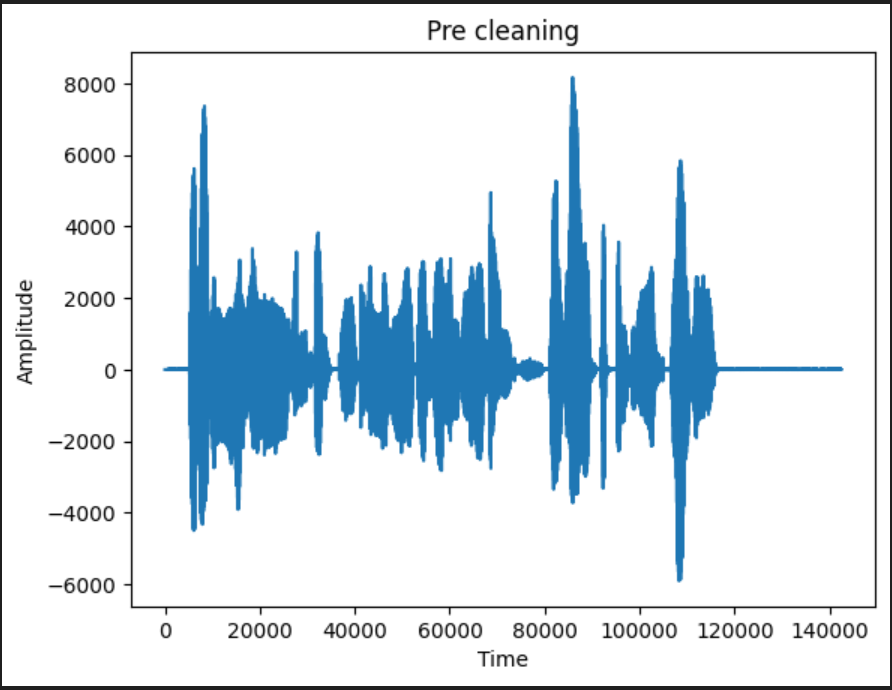
\includegraphics[width=\linewidth]{images/pre_cleaning.png}
        \caption{Figure 2}
        \label{fig:image2}
    \end{subfigure}
    \hfill
    \begin{subfigure}[b]{0.3\textwidth}
        \centering
        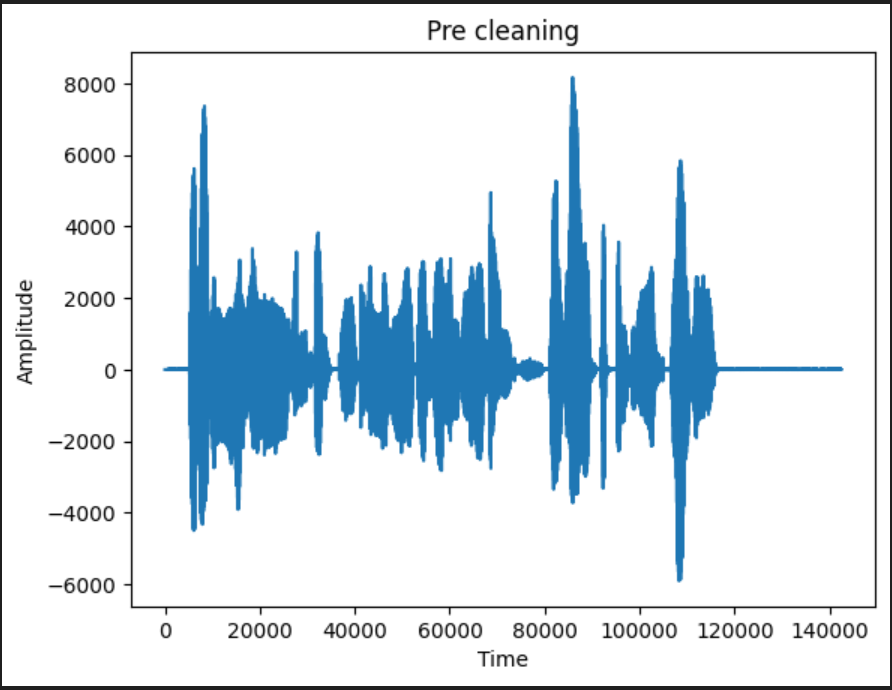
\includegraphics[width=\linewidth]{images/pre_cleaning.png}
        \caption{Figure 3}
        \label{fig:image3}
    \end{subfigure}
    \caption{Three aligned images with individual captions}
    \label{fig:three_images}
\end{figure}\\
By looking at the count, some languages are overrepresented in our data, which is not ideal because it can lead to a model that is biased towards these languages, potentially reducing its performance on underrepresented languages. Furthermore, we can see that the average length of the samples for each are very heterogeneous, ranging from 2 seconds to 5 seconds. This would need to be kept in mind when producing the features from the soundwaves, so the windows properly capture lengths of each file. That being said, by looking at the total length of audios, which is the sum of seconds spoken for each language, we see that the difference between languages is slightly smaller. Overall, we see some unbalancing in our labels. Knowing this, we will need to stratify the dataset when doing the train/test splits so that each language is proportionately represented in the train and test sets, ensuring a more balanced and accurate evaluation of the model's capabilities across all languages.

\subsection{Data Preprocessing}
For the preprocessing of audio data, we use different features which are presented below. These features were picked to produce a holistic representation of spoken languages, covering a wide range of language features. Given that 

\textbf{MFCCs}:
The Mel Frequency Cepstral Coefficients (MFCCs) are criticals in the sense that it allows capturing the different aspects that are unique to each spoken language. It is much easier to differentiate languages by using MFCCs. In our case, we decomposed our audio data using $512$ samples from each audio file. With a sample rate of $16000$ we get windows of length $0.032$ milliseconds. Furthermore, we set the number of MFCCs to be $25$, as recommended for spoken language. We yield, for each data point, a matrix $M \in \R^{25 \times n}$, where $n$ is the number of windows. We then compute a vector $V \in \R^{25}$ from $M$, where each element is this mean of an MFCC. These $25$ features are added to the final attribute matrix. 
%To obtain the MFCCs, we first found the spectrum of power as a function of our audio file's frequencies from a Fast Fourier Transformation (FFT). Then, it was necessary to find the Mel Filter Banks (MFB) of the spectrum from which we obtain the frequency energies (weighted energy) passing through each filter of the bank. A logarithmic function will be applied to these energies. Finally, by applying a Discrete Cosine Transformation on the log-transformed energies, we obtain the MFCCs.\\

\textbf{Spectral Centroid}: The spectral centroid indicates the center of mass of the sound's spectrum, providing a way to characterize the brightness of a sound. It is calculated as the weighted mean of the frequencies present in the signal, with their magnitudes as the weights. We yield a vector $V \in \R^{n}$ where $n$ is the number of windows. To have a standardized format to add in our attribute matrix, we compute mean, median, standard deviation, $25th$ percentile, $75th$ percentile, maximum value, and minimum value, from $V$ for each data point. This transformation is applied to all the spectral features (spectral rolloff and spectral bandwidth). 

\textbf{Spectral Rolloff}: The spectral rolloff point indicates the frequency below which a specified percentage of the total energy of the spectrum is located, typically used to distinguish between harmonic (tonal) and noisy sounds. It serves as a way to capture the shape of the sound's spectrum, particularly its high-frequency content.

\textbf{Spectral Bandwidth}: Spectral bandwidth quantifies the width of the frequency band where most of the sound's energy is concentrated, reflecting the sound's perceived texture. It measures the spread of the spectrum around the spectral centroid, indicating the range of significant frequencies that contribute to the sound.

\textbf{Pitch and Intonation Patterns}: Pitch refers to the perceived frequency of a sound, determining the musical note or tone that it corresponds to. Intonation pattern describes the variation of pitch over time within spoken language, contributing to the expression of emotions, questioning, or emphasis in speech. Each data point produces a matrix $P \in \R^{n \times m}$ of pitch tracks and a matrix $M \in \R^{n \times m}$ of magnitude windows, where each line represents a the pitch track or magnitude of a given window. From these matrices, we produce a vector of size $V \in \R^{n}$ where each element is the pitch with the most magnitude for each window (windows that only have null pitches are dropped). From $V$ we compute, the mean, median, standard deviation, $25th$ percentile, $75th$ percentile, maximum value, and minimum value, from $V$ which is then added to our attribute matrix. 

\textbf{Formant Frequencies}: 
%In audio processing, a formant is a concentration of acoustic energy around a particular frequency in the voice spectrum, associated with the resonant frequencies of the vocal tract. 
A formant is a characteristic component of the quality of a speech sound, particularly a vowel. When we speak, our vocal tract acts as a resonator, emphasizing specific frequencies and shaping the sounds we produce. Formants play a crucial role in characterizing vowels and certain consonants, greatly influencing speech recognition and synthesis. We will focus on three types of formants, which will be extracted using the \textit{parselmouth} library. \textit{F1} which is determined primarily by the height of the tongue body, \textit{F2} influenced by the frontness or backness of the tongue body,  \textit{F3} which is associated with lip rounding. For each data point, we extract \textit{F1}, \textit{F2}, \textit{F3} values for a set time point. Given that the lengths of our data points aren't the same, we compute the habitual mean, median, standard deviation, $25th$ percentile, $75th$ percentile, maximum value, and minimum value, for each type of formant. We also extract the difference between the means of \textit{F1}, \textit{F2}, \textit{F3}, yielding two additional features. These values are then added to the attributes matrix. 

\textbf{Root Mean Square (RMS)}: Root Mean Square (RMS) represents the square root of the average power of a signal, providing a measure of its amplitude. It's commonly used to quantify the volume level or energy of an audio signal over time. We compute the RMS energy for each frame, yielding a vector $v \in \R^{n}$, where $n$ is the number of windows. From $v$, we compute the habitual central tendency metrics (as cited above), interquartile range, the energy variability (sum of absolute differences), and low-energy frame rate ()

\textbf{Zero Crossing Rate (ZCR)}: Zero crossing rate (ZCR) is the rate at which an audio signal changes from positive to negative or back, effectively measuring the number of times the amplitude crosses the zero point. This feature is useful for analyzing the noisiness of a signal and distinguishing between voiced and unvoiced speech. We retrieve a vector $v \in \R^{n}$ where $n$ is the number of windows, and where each element is the fraction of zero crossings in a given window.

\textbf{Harmonics to Noise Ratio (HNR)}:
Harmonics to noise quantifies the amount of harmonic sound (periodic vibrations) relative to the amount of noise (non-periodic components) in a voice signal. A higher HNR generally indicates a clearer and more harmonic sound, which is often associated with a healthier and more typical voice production. In our case, we compute the HNR mean (represented in decibels) from all the audio clips, using the \textit{parselmouth}. This value is then added to the attribute matrix. 

\section{Methodology}
\subsection{Why supervised Learning ?}
Supervised learning algorithms (SVM and Random forest) are used in this project because unlike unsupervised learning algorithms, they learn the specific characteristics of each language’s phonetic, intonational, and rhythmic properties, leading to highly accurate classification once the model is well-tuned. Unsupervised methods like clustering algorithms (DBscan, K-means or hierarchical clustering) identify groups based on feature similarity but do not inherently know what these groups represent (which language each group corresponds to) which can lead to an ambiguity in cluster interpretation.

Unsupervised algorithms suffer more from the curse of dimensionality than supervised models. In fact, SVMs are more effective even in hight dimension due to the fact that they primarily care about the points closest to the decision boundary (support vectors) rather than the dimensionality of the space. Furthermore, the maximization of the distance between the support vectors and the boundary ensures that the model focuses on the most informative features for classification. This property allows SVM to be less prone to overfitting, a common issue in high-dimensional spaces. Due to the kernel trick, SVMs can also handle non linear decisions which allows them to operate in higher dimensions without directly computing the coordinates in that space unlike DBscan or k-means for example (more description about SVM on the section \textbf{4.3}).

In other hands, random forest is based on a set of decision trees which are robust against overfitting because each tree in the forest is bult from a random sample of features, reducing the variance of the set without substantially increase the biais. Furthermore, the classification for random forest is more efficient in hight dimensionality compared to unsupervised algorithms because it randomly selects subsets of features at each split, which means it can manage high-dimensional data by focusing on the most informative features for making splits.


\subsection{Dimensionality reduction}
Before applying PCA (Principal Component Analysis) or MDS (Multi-Dimensional Scaling), we wanted to see the relationship between features i.e. how strongly they are correlated. This correlation study would guide us in the dimensionality reduction algorithm we choose to apply to our data. If some features are strongly correlated, PCA would be pertinent to be applied, as some features are linearly related. Even though our correlation study (see the correlation matrix in the result section) gave us pretty strong evidence of non-linear relationship between our features (meaning that MDS might be a better suit for our dataset), we opted to reduce dimensionality using PCA due to insufficient computing and memory.

The PCA method searches for an orthogonal projection of the original data, minimizing the mean squared error over the dataset. 

After applying PCA, with a maintained variance of $95\%$, we have $90$ features from the $161$ initial features. This means that the first $90$ principal components of the covariance matrix $\Sigma \in \mathbb{R}^{151 \times 151}$ , capture $95\%$ of the variance in the original training set.

\subsection{Support Vector Classifier}
For this project, we use the library \textit{SVC} from \textit{sklearn} for multi-class classification. It trains an SVM one-vs-one classifier for each pair of classes, and then builds from them a one-vs-rest classifier for each class. The single class prediction is obtained from the most confident prediction of the one-vs-rest classifiers. 

This library use a non-linear SVM with a soft margin. Non-linear SVM with a soft margin is particularly useful when dealing with data that cannot be linearly separated in the original feature space (which is the case in our situation). The inclusion of slack variables, \(\xi_i\), allows some data points to be on the incorrect side of the margin, providing a balance between the complexity of the model and its error minimization.\\

\textbf{Mathematical formulation}

For a dataset $X \in \R^{n \times p}$ and a vector $y \in \{-1, 1\}^n$, the objective is to find $w$ such that the values returned by the functions $f(X) = sign(w^T\phi(x) + b)$ are correct for most samples.\\
\textit{SVC} resolve the following primal problem : \(\displaystyle
\min_{w, b, \boldsymbol{\xi}} \left( \frac{1}{2} w^T w + \beta \sum_{i=1}^{n} \xi_i \right)
\) 
subject to:\\
\( y_i (w^T \phi(x_i) + b) \geq 1 - \xi_i\), \(\xi_i \geq 0, \quad \forall i\).
By using Lagrange multipliers, we obtains the dual :\(\displaystyle \min_{\alpha} \frac{1}{2} \alpha^T Q \alpha - \mathbf{1}^T \alpha
\) subject to: \(y^T \alpha = 0\), \(0 \leq \alpha_i \leq \beta, i=1,...,n\) with $Q$ an $n$ by $n$ positive semidefinite matrix, $Q_{ij} \equiv y_iy_jK(x_i, x_j)$, where $K(x_i, x_j) = \phi(x_i)^T\phi(x_j)$ is the kernel. 

After the optimisation is done, the output for the decision function for $X$ is :\(\displaystyle \sum_{i\in SV} y_i\alpha_i K(x_i, x) + b\)
where $SV$, represent the support vectors (the points that lies within the margin).

\textbf{Hyperparameters}\\
When tuning our model, we considered three hyperparameters to tune, the regularization parameter for the soft margin $\beta$, different types of kernels, and their scale coefficient. As mentionned previously, slack variables allow some points to be on the wrong side of the margin. We can intuitively see that if there is no constraint on the slack variables, the model will be too lenient, meaning that it will accept too many incorrect classifications. The $\beta$ regularization parameter will modulate the slackness of the margin. The higher the value of $\beta$, the slacker, and the more lenient, is the margin. \\
For the kernels ($\gamma$ parameter that is included in the kernel definitions), we test a polynomial kernel, rbf kernel, and a linear kernel. The linear kernel, defined as $K(x, y) = x^T y$ where $x$ and $y$ are feature vectors, assumes that the boundaries between classes is a linear function in the $\R^n$ space. Knowing that our data is most likely non-linear given our correlation study, we didn't have much hope that this kernel would yield good results, but we still added it to our kernel set to compare to the other intuitively more promising kernels. The polynomial kernel defined as, $K(x, y) = (\gamma x^T y + r )^d$, where $\gamma$ is a scale factor that controls the influence of higher-order terms in the polynomial, $r$ is a constant, and $d$ is the degree of the polynomial. This kernel represents the similarity between vectors in a feature space over polynomials of the original data. The rbf kernel, defined as $K(x, y) = exp(\gamma \| x - y \|^2)$, with $\gamma$ defines how much influence a single training example has on the fitting of the model. The larger $\gamma$ is, the closer data points must be to affect the model significantly, and thus, preventing from overfitting. The RBF kernel maps samples into a higher dimensional space using the square of the Euclidean distance between them, and thus it is very effective in cases where the decision boundary is highly irregular and cannot be approximated by a simple hyperplane. \\
Having briefly defined the $\gamma$ parameter, let's delve into more detail into how it affects the polynomial and RBF kernels respectively. The $\gamma$ parameter plays a critical role in defining the behavior of both the polynomial and RBF kernels, each in a distinct manner, tailored to their specific mathematical formulations.
For the polynomial kernel, $\gamma$ serves as a scaling factor for the dot product \(x^T y\) in the formula $(K(x, y) = (\gamma x^T y + r)^d)$. By adjusting $\gamma$, we control the influence of higher-order terms in the polynomial. Increasing $\gamma$ emphasizes the higher degrees of the polynomial, thereby capturing more complex patterns in the data, but also increasing the risk of overfitting, especially in noisy datasets or those with outlier points. Conversely, a lower $\gamma$ reduces the complexity of the model, making it behave more linearly, which could be beneficial for datasets where the underlying patterns are less complex. In our case, we would need a high value of $\gamma$ given the complexity of our data.

In the case of the RBF kernel, $\gamma$ impacts the width of the Gaussian function used to measure the similarity between points: $(K(x, y) = \exp(-\gamma \| x - y \|^2))$. A high $\gamma$ value results in a narrow peak, meaning that only data points close to each other are considered similar. This sensitivity allows the model to fit closely to the training data, which can capture intricate data structures but may lead to overfitting if the data has noise. A lower $\gamma$ produces a wider peak, giving the model a more general perspective of the data, enhancing its ability to generalize but potentially underfitting complex datasets.


\begin{comment}
\textbf{Kernel Function}\\
Common choices for the kernel function \(K\) include:
- Polynomial: \(K(\mathbf{x}_i, \mathbf{x}_j) = (\gamma \mathbf{x}_i^T \mathbf{x}_j + r)^d\),
- Radial Basis Function (RBF): \(K(\mathbf{x}_i, \mathbf{x}_j) = \exp(-\gamma \|\mathbf{x}_i - \mathbf{x}_j\|^2)\),
- Sigmoid: \(K(\mathbf{x}_i, \mathbf{x}_j) = \tanh(\gamma \mathbf{x}_i^T \mathbf{x}_j + r)\).
\(\gamma\), \(r\), and \(d\) are parameters that can be tuned according to the specific data and problem requirements.  
\end{comment}


\subsection{Random Forest}
For this project, we use the library \textit{RandomForestClassifier}(RFC) from \textit{sklearn}.
Random Forest is an ensemble learning technique that builds multiple decision trees and merges them together to get a more accurate and stable prediction. The algorithm combines the output of multiple (often hundreds) randomly created decision trees, a method known as \textit{bootstrap aggregating}, or \textit{bagging}. Each tree in the forest is built from a sample drawn with replacement (i.e., a bootstrap sample) from the training set.

\textbf{\large Mathematical Description}

Let \( \mathcal{D} = \{(X_1, Y_1), (X_2, Y_2), \dots, (X_n, Y_n)\} \) be a dataset containing \( n \) samples, where each sample consists of a feature vector \( X_i \) and a corresponding label \( Y_i \). Random Forest creates a multitude of decision trees using the following steps:

\begin{enumerate}
    \item For each tree, a random sample of \( m \) features is selected from the total \( p \) features.
    \item Each tree is grown to the fullest extent possible and no pruning is performed.
    \item The output of the Random Forest is given by the mode of the classifications (for classification tasks) or the mean prediction (for regression tasks) of the individual trees.
\end{enumerate}

Mathematically, the prediction of a Random Forest classifier can be expressed as:

\begin{equation}
    \hat{Y}^p = \frac{1}{N_T} \sum_{b=1}^{N_T} T_b(X)
\end{equation}

where \( N_T \) is the number of trees in the forest and \( T_b \) represents the prediction of the \( b \)-th tree.

\textbf{\large Hyperparameters}

The performance of a Random Forest model is highly dependent on the settings of various hyperparameters. Here, we discuss some of the most crucial ones:

\begin{itemize}
    \item \texttt{n\_estimators}: It specifies the number of trees in the forest. More trees increase the model's accuracy and stability by reducing the variance in predictions, but they also increase computational demands. Generally, there are diminishing returns in performance improvement beyond a certain number of trees.

    \item \texttt{criterion}: The impurity measure used when splitting tree nodes. Each decision split chooses the predicate condition that minimises the expectation of this measure on the sub-populations divided among sub-trees. \\
    First, the Gini score \( \displaystyle G(p_1 \dots p_k) = 1 - \mathbb{E}_k[p_k]\). In words, that is the average probability of not finding each class. \\
    Second, the entropy \(\displaystyle H(p_1 \dots p_k) = \mathbb{E}_k[-\log_2 (p_k)]\) measures the uncertainty in bits 
    These impurity measures are minimised when there is only one class found in a sub-tree's population. They are maximised when all classes are found in equal amounts.

    \item \texttt{max\_depth}: The maximum depth allowed for each tree. A deeper tree can model more complex relationships by creating more specific rules. However, it also makes the model more likely to overfit to the noise in the training data.

    \item \texttt{min\_samples\_split}: The minimum number of samples required to split an internal node. Higher values prevent the model from learning overly specific patterns, thus lowering the risk of overfitting. Smaller values allow the trees to make more complex decisions, increasing the risk of overfitting.

    \item \texttt{min\_samples\_leaf}: The minimum number of samples required to be at a leaf node. Setting this parameter can ensure that leaf nodes contain more than one sample, which helps in smoothing the model's predictions and preventing overfitting.

    \item \texttt{max\_features}: The number of features to consider when looking for the best split. Increasing `max\_features` generally improves the performance of the model as each node now has a higher number of options to consider. However, this can also increase the correlation between the trees, reducing model variance but potentially increasing bias.

    \item \texttt{bootstrap}: Whether bootstrap samples are used when building trees. If False, the whole dataset is used to build each tree. Using the default bootstrapping adds randomness to the model, by training each tree on a random subset of the data, which helps in reducing model variance and avoiding overfitting.
    
\end{itemize}
\subsection{Hyperparameter Tuning}
Hyperparamter tuning is a crucial step to finding the best model. As data our data is complex and highly dimensional, we will need to apply a hyperparameter tuning to find the best parameters of our models (SVC and RFC). We will use a Random Search algorithm to find the best hyperparameters (see Algorithm 2). A Grid Search would've been another alternative, which would exhaustively search for the best model in a given hyperparameter space.   

\begin{algorithm}
\caption{Random Search with Cross-Validation}
\begin{algorithmic}[1]
\State Initialize dataset $D$
\State Define set of hyperparameters $H$
\State Initialize best performance as $-\infty$
\State Initialize best hyperparameters as $\emptyset$
\For{each set of hyperparameters $h \in H$}
    \State Split $D$ into 5 equal folds $D_1, D_2, D_3, D_4, D_5$
    \State Initialize performance list $P$
    \For{$i \gets 1$ to $5$}
        \State Set $D_{\text{train}} \gets D \setminus D_i$ (all folds except the $i$-th fold)
        \State Set $D_{\text{test}} \gets D_i$
        \State Train a RFC model on $D_{\text{train}}$ with hyperparameters $h$
        \State Evaluate the model on $D_{\text{test}}$ and store the performance in $P$
    \EndFor
    \State Compute mean performance $m \gets \text{mean}(P)$
    \If{$m > \text{best performance}$}
        \State Update best performance $ \gets m$
        \State Update best hyperparameters $\gets h$
    \EndIf
\EndFor
\State Output the best hyperparameters
\end{algorithmic}
\end{algorithm}

\section{Results}
For the sake of consistency and reproducibility, we fixed the "random\_state" parameter of all training components: \\
- The data splitter deciding which vectors are part of the overall training vs test set. \\
- The dimension reduction operators PCA and MDS. \\
- The classifier models SVC and RandomForestClassifier. \\
- The hyper-parameter optimizer RandomizedSearchCV.

\subsection{Rejected methods}
In this section, we talk about the methods that we tried but didn't work. Based on the correlation matrix in the appendix, we can see that our data are not well correlated. So, it is more relevant to use MDS instead of PCA but MDS demand more computational resources. We tried to reduce the dimensionality with MDS, both with euclidian or malahanobis distance, but our Python environments crashed due to insufficient memory. Maybe the number of data points was too high at $\sim22$k. This happened also on the cloud Colab environment. 
In fact, MDS involves computing the distances between all pairs of points in the dataset and then optimizing the configuration of points in the new space to reflect these distances as closely as possible.

The \textit{Common Language} dataset we are using came pre-separated into a 'train', 'test' and 'validation' set. Initial training runs with this split gave very poor results ($\approx$ 2x worse), compared to random selections from the whole dataset. So, we decided to use \textit{sklearn}'s stratified splitter on the entire dataset, ignoring the pre-defined split. Stratification ensures that the chosen subsets contain the same proportions of each class label.

\begin{table}[h]
    \centering
    \begin{tabular}{|c|c|c|c|c|}
    \hline
      Models & Accuracy & f1-score & Precision & Recall\\  
      \hline
      SVC & 13.61\% & 12.64\% & 12.91\% & 13.17\%\\
        \hline
      RFC & 10.99\% & 8.75\% & 9.81\% & 10.22\% \\
    \hline
    \end{tabular}
    \label{tab:my_label}
    \caption{With the \textit{Hugging Face} data split}
\end{table}

In the initial datasets, we have 45 labels. Some languages in the labels are very similar so we reduced the number of labels by grouping them based on the region in which they are spoken. We used GPT-4 to find new labels. Here is the promp we used : \texttt{We have a set of labels for a classification task based on speech and want to relable them based on similarity and geographic location. Output 10 new labels.}

Here is the comparaison of the results after running the models (with the best hyperparameters) with 45 labels vs 10 labels:
\begin{table}[h]
    \centering
    \begin{tabular}{|c|c|c|c|c|}
    \hline
      Models & Accuracy & f1-score & Precision & Recall\\  
      \hline
      SVC & 24.60\% & 23.35\% & 24.08\% & 23.61\% \\
        \hline
      RFC & 17.91\% & 16.20\% & 17.12\% & 17.06\% \\
    \hline
    \end{tabular}
    \label{tab:my_label}
    \caption{With 45 labels}
    
    \centering
    \begin{tabular}{|c|c|c|c|c|}
    \hline
      Models & Accuracy & f1-score & Precision & Recall\\  
      \hline
      SVC & 29.82\% & 29.66\% & 29.72\% & 29.66\%\\
        \hline
      RFC & 26.48\% & 25.36\% & 28.51\% & 25.50\% \\
    \hline
    \end{tabular}
    \label{tab:my_label}
    \caption{With 10 labels}
\end{table}

Given that the data has less labels (is less complex), the models learn better which explain why the metrics increased. There is less room for misclassification.

\subsection{Metrics}
In order to compare, and determine the best model, we need to set metrics which will guide us to our decision. We will use four metrics, accuracy, F1 scores, precision and recall. These metrics are defined in terms of hte number of sample and the four categories. True/False means that the classifier is right or wrong and Positive/Negative means that the classifier predicts that the sample is in the class +/- resp. So a \textit{True Positive} represent the fact that the classifier predicts that a sample is in the + class and he is right. A \textit{False Positive} represent the fact that the classifier predicts that a sample is in the + class but he is wrong. And the same logic goes for \textit{True Negative}  and \textit{False Negative}.

\textbf{Accuracy:} The accuracy of a classifier is the ratio between the number of True positives and the total number of predictions ($P(Class == Prediction)$): 

\(\displaystyle \text{Accuracy} = \frac{\text{True Positive + True Negative}}{\text{Total number of predictions}} \)

\textbf{Precision score:} The precision of a classifier represent the probability that the sample is really in the class + knowing that the classifier prediction is + ($P(Class=+ | Prediction = +)$). The is the probability that the prediction of the classifier is right:

\(\displaystyle \text{Precision} = \frac{\text{True Positive}}{\text{True Positive + False Positive}}\)

\textbf{Recall score:} The recall is the probablity that the prediction of the classifier is + knowing that the sample is really in the class + ($P(Prediction=+ | Class = +)$):

\(\displaystyle \text{Recall} = \frac{\text{True Positive}}{\text{True Positive + False Negative}}\)


\textbf{F1 Score:} This metric is (almost) the Jaccard similarity between the sets of positive classification and positive prediction. That would be the ratio of their intersection over their union. 
$$\frac{P(Prediction=+ \land Class = +)}{P(Prediction=+ \lor Class = +)}$$
But instead, F1 score is twice the intersection, divided by the union plus the intersection again.
$$\frac{2 \times P(Predict =+ \land Class = +)}{P(Class = +) +  P(Predict=+)}$$
It can be calculated as the harmonic mean of Precision and Recall:

\(\displaystyle \text{F1} = \frac{2}{\frac{1}{\text{Precision}} + \frac{1}{\text{Recall}}} \displaystyle = 2 \times \frac{\text{Precision}\times\text{Recall}}{\text{Precision + Recall}} \). 

\subsection{SVM}
After cleaning our data and training the models with no hyperparameters tuning, we get those results:

\begin{table}[h]
    \centering
    \begin{tabular}{|c|c|c|c|c|}
    \hline
      Kernel & Accuracy & f1-score & Precision & Recall\\  
      \hline
      Linear & 19.75\% & 18.42\% & 18.49\% & 19.01\%\\
        \hline
      Poly & 19.02\% & 17.91\% & 26.08\% & 17.74\% \\
        \hline
      RBF & 24.54\% & 16.20\% & 23.02\% & 22.54\% \\
    \hline
    \end{tabular}
    \label{tab:my_label}
    \caption{Results before grid search}

\end{table}

Then, applying random search (Algorithm 2) gives us those parameters : \texttt{C=10, gamma=auto, kernel=rbf} and we get these results after training a SVM with those hyperparameters:


\begin{table}[h]
    \centering
    \begin{tabular}{|c|c|c|c|c|}
    \hline
      Kernel & Accuracy & f1-score & Precision & Recall \\
      \hline
      RBF & 24.60\% & 23.35\% & 24.08\% & 23.61\% \\
    \hline
    \end{tabular}

    \label{tab:my_label}
    \caption{Results after grid search}
\end{table}

\subsection{Random Forest}
As an exploratory first step, we fitted our data to an Random Forest Classifier, with sklearn's default hyperparameters. Here are the results:

\begin{table}[h]
    \centering
    \begin{tabular}{|c|c|c|c|}
    \hline
      Accuracy & f1-score & Precision & Recall \\
      \hline
      17.91\% & 16.20\% & 17.12\% & 17.06\% \\
    \hline
    \end{tabular}

    \label{tab:my_label}
    \caption{Results before grid search}
\end{table}

We applied a Random Search algorithm (Algorithm 2) to find the best hyperparamters in a given hyperparameter space. The output of this search gave us this set of hyperparameters \texttt{n\_estimators = 200, min\_samples\_split = 5, min\_samples\_leaf = 4, max\_features = sqrt, max\_depth = None, criterion = gini} which yield the best . Results obtained after running the Random Search : 




In both SVC and RFC, we see an improvement in all of our metrics after running the Random Search. This suggests that by exhaustively exploring the hyperparamter space, we could potentially find an even better model (even though the performance gain is marginal).  

\begin{table}[h]
    \centering
    \begin{tabular}{|c|c|c|c|}
        \hline
         Accuracy & F1-score & Precision & Recall\\
        \hline
         20.57\% & 17.90\% & 20.96\% & 19.51\%\\
        \hline
    \end{tabular}
    
    \label{tab:my_label}
    \caption{Results after grid search}
\end{table}

\section{Conclusion}
This project embarked on the challenge of comparing the efficacy of two widely used machine learning algorithms, Support Vector Machines (SVC) and Random Forests (RFC), in the domain of language classification based on speech. Through extensive data preprocessing, model training, and hyperparameter optimization, several key insights were unearthed.

Firstly, the reduction of labels from 45 to 10, intended to simplify the classification problem, yielded expected results. Both SVC and RFC metrics increased do to the reduce of the complexity of the label set. So, both algorithm demonstrated robustness by improving accuracy when the problem space was reduced, underscoring its adaptability to variations in data complexity.

Moreover, the process of hyperparameter tuning was pivotal, showcasing significant improvements in model performance. It emphasized the importance of algorithm-specific parameter settings, which tailored each model more closely to the intricacies of the task.

We can also see that SVC f1-score is 30\% higher than RFC. So globaly, based on the results obtained in this project, we can conclude that SVC is a better classifier.

In conclusion, this project not only reinforced the necessity of careful data preprocessing and the strategic choice of model parameters but also illuminated how different algorithms can uniquely respond to changes in data structure. For future work, exploring additional ensemble techniques, and possibly integrating more advanced neural network architectures, could provide further enhancements in the field of language classification. The insights gained here lay a foundation for deeper exploration into automated language recognition, promising to elevate the tools available for global communication and information exchange.

\section{Team Contributions}
\textbf{Samir:} Has done all the project alone.

\textbf{Kamen:} Nothing.

\textbf{Simon:} Nothing.

\end{document}